\documentclass[journal,compsoc,10pt]{IEEEtran}

% Load some possibly useful packages. You can remove the ones you don't need or
% add other packages that you need in your paper.
\usepackage{graphicx}                   % required to include graphics
\usepackage{amsfonts,amssymb,amsmath}   % mathsymbols etc
\usepackage{mathtools}                  % includes some fixes to amsmath, and adds convenience macros
\usepackage{bm}                         % make any letter boldface in math
\usepackage{algpseudocode}              % aka `algorithmicx`: same look `algorithmic`, but more flexible
\usepackage{array}                      % for better looking arrays
\usepackage{booktabs}                   % for better looking tables
\usepackage[usenames]{xcolor}           % colors for highlighting etc.
\usepackage{url}                        % for urls
\usepackage[%pdftitle=,                 % define the PDF metadata
            %pdfauthor=,
            colorlinks=true, linkcolor=purple, urlcolor=blue, citecolor=cyan,
            anchorcolor=black   % make links/references 'clickable' without ugly frames
            ]{hyperref}            
\usepackage[capitalise]{cleveref}                   % smart references to figures, equations etc.

% some packages which may be useful when drafting, but should be removed before submission
\usepackage{todonotes}

%own packages
\usepackage{amsthm}
\usepackage{float}
\usepackage{tkz-graph}
\usepackage[table]{xcolor}
\usepackage{subcaption}
\usepackage{pgfplots}
\usepackage{pgfplotstable}

\pgfplotstableset{
    color cells/.style={
        col sep=comma,
        string type,
        postproc cell content/.code={%
                \pgfkeysalso{@cell content=\rule{0cm}{2.4ex}\cellcolor{black!##1}\pgfmathtruncatemacro\number{##1}\ifnum\number>50\color{white}\fi}%
                },
        columns/x/.style={
            column name={},
            postproc cell content/.code={}
        }
    }
}

% You can define your own commands. This is useful for shorthands, for example
\newcommand{\EE}{\mathbb{E}}
\newcommand{\RR}{\mathbb{R}}
\newcommand{\CC}{\mathbb{C}}
\newcommand{\NN}{\mathbb{N}}
\newcommand{\eE}{\mathcal{E}}
\newcommand{\gG}{\mathcal{G}}
\newcommand{\gS}{\mathcal{S}} %sinks
\newcommand{\nN}{\mathcal{N}}
\newcommand{\lnorm}[1]{\ell_{#1}\text{-norm}}

% Commands are also useful to ensure standardized notation, such as how to display vectors and matrices.
% The point is to replace formatting commands with semantic ones.
% This both makes the source more semantic, and also makes it easier to change formatting choices later
% IMPORTANT: In TeX, all commands share a global namespace. You need to be careful therefore not to overwrite an existing command.
%            Use \newcommand to ensure you don't accidentally overwrite an important macro
%            Use \renewcommand if you *do* want to overwrite a macro, have checked what the original does,
%            and have made sure the redefinition is safe.
\newcommand{\T}{\mathsf{T}}            % transpose
\renewcommand{\vec}[1]{\bm{#1}}        % redefine \vec to produce boldface instead of adding an arrow
\newcommand{\mat}[1]{\bm{#1}}          % define \vec to produce boldface
\newcommand{\ones}{\bm{1}}             % all-ones vector
\newcommand{\zeros}{\bm{0}}             % all-ones vector
\newcommand{\zerosmatr}{\bm{0_{n\times n}}}
\newcommand{\onessmatr}{\bm{1_{n\times n}}}     % all-zeros matrix
\newcommand{\eye}{\bm{I}}              % identity matrix
\newcommand{\ei}{\bm{e}_i}             % standard basis vector e_i
\newcommand{\ej}{\bm{e}_j}             % standard basis vector e_j
    % TIP: Resist the temptation to be too clever with macros
    %   - \ei and \ej are easier to type than e.g. \ee[i]  (note that \e is a low-level command and should not be redefined)
    %   - While you can define macros in terms of other macros  (eg we could define \ei in terms of \vec),
    %     many journals won’t accept this. Recursive macros also produce more frequent and more complicated compilation errors

% eigene libs
\newtheorem{theorem}{Theorem}[section]
\newtheorem{corollary}{Corollary}[theorem]
\newtheorem{lemma}{Lemma}[section]
\newtheorem{definition}{Definition}[section]
\usepackage{enumitem}

% Commands like \sin and \exp ensure proper fonts and spacing for math operators.
% Use the dedicated \DeclareMathOperator to define new operators
\DeclareMathOperator{\diag}{diag}

\begin{document}%[tikz,border=3mm]{standalone}
%\usetikzlibrary{arrows.meta,positioning,quotes}

\title{Opinion Formation on Networks: The DeGroot Model and Its Extensions}

% author information
% COMMENT OUT THESE LINES FOR YOUR CONFERENCE SUBMISSION!
\author{Jesper Nilsson, 457057}

\maketitle
\thispagestyle{plain}
\pagestyle{plain}

\begin{abstract}
    % Understanding how opinions emerge and evolve within a population is central to explaining collective behavior and social dynamics. 
    In this paper, we take a closer look at the DeGroot model (1974) and analyze its convergence and network properties. We show that if the weight matrix $\mat A$ is primitive, then the model converges to a consensus. We also prove that this condition can be verified by checking whether the corresponding graph is strongly connected and aperiodic. Moreover, we show that the connectedness of the graph provides an upper and lower bound for the second largest eigenvalue of $\mat A$, which in turn gives us an upper bound for the convergence speed of the model. Finally, we take a look at the Friedkin-Johnsen model (1990, 1999) and the Hegselmann-Krause model (2002). For the former, we show that the model converges if the product $\mat D\mat A$ of the \textit{susceptibility} matrix $\mat D$ and $\mat A$ is irreducible. For the latter, we provide a condition that ensures the convergence of the model. To explain the concepts, we provide some independent proofs and observations.
\end{abstract}


\section{Introduction}
As individuals interact and exchange views, local patterns of agreement or disagreement can propagate through social networks, leading to large-scale outcomes such as consensus, polarization, or fragmentation. The question of how, for example, echo chambers form and influence opinions is a strongly debated topic in our society.

In order to better understand these phenomena, many attempts have been made to analyze and model the formation of opinions, like the voter model \cite{Voter-model}, Ising model \cite{Ising-model}, Friedkin and Johnsen model \cite{Friedkin01011990} and Hegselmann-Krause model \cite{Hegselmann-Krause}. Another well-known example is the DeGroot model \cite{Degroot01031974} which presents a rather simple, iterative process (see in \cref{sec:degroot}).
Given an instance of this model, we can then analyze or calculate properties such as whether the group will reach a consensus, what consensus they reach, and how fast they will reach it (see in \cref{sec:Convergence_properties}). Moreover, the model can be represented and visualized as a graph with the nodes and edges representing who is communicating with whom. Thereby, we can use features of these graphs as conditions and explanations for the aforementioned properties (see in \cref{sec:network_prop}).

As the DeGroot model is a rather simple abstraction of opinion formation in real social networks, it does not capture all aspects of social interaction. Therefore, we will take a look at two extensions of the DeGroot Model (see in \cref{sec:extensions}). First, the Friedkin-Johnsen model and second, the Hegselmann-Krause model.

% Subject --> Parameter
% subjective distribution <-- opinion
\section{Preliminaries and Notation}\label{sec:prelim_notation}
In this paper, we use $\ones$ to denote the vector with all-ones and $\eye$ to denote the identity matrix. Similarly, the vector with all-zeros is referred to as $\zeros$. For a given vector $(.)^\T$ denotes the transpose of the vector. We use the following style for vectors $\vec p$, matrices $\mat M$, and graphs $\gG$. Moreover, $V(\gG)$ denotes the set of vertices and $E(\gG)$ the set of edges in $\gG$. For a matrix $\mat M$, the notation $(\mat M)_{ij}$ refers to the entry in the $i$-th row and $j$-th column of $\mat M$. Furthermore, we use the notation $\underline{n} = \{1,\dots,n\}$. 

A row-stochastic matrix $\mat A \in [0,1]^{n\times n}$ is defined, such that all its entries are non-negative and its row vectors sum up to 1, i.e., $\sum_{j=1}^na_{ij} = 1$ for all $i \in \underline{n}$. A row-substochastic matrix $\mat A \in [0,1]^{n\times n}$ is a non-negative matrix for which all row vectors sum up to at most 1 and at least one row vector sums up to less than 1, i.e., $\sum_{j=1}^na_{ij} \leq 1$ for all $i\in \underline{n}$ and $\sum_{j=1}^na_{ij} < 1$ for at least one $i\in \underline{n}$. Furthermore, a digraph describes a directed graph, meaning every edge has a direction. A graph is strongly connected if and only if every node $v \in V(\gG)$ is reachable from every other node $u \in V(\gG)$ (with $v \neq u$), i.e., there exists a directed path from every node $u$ to $v$. A sink $\gS$ is a strongly connected subgraph, i.e., $V(\gS) \subset V(\gG)$ and $E(\gS) \subset E(\gG)$, that has no node $i\in V(\gS)$, such that there exists a node $j\notin V(\gS)$ with $(i,j)\in E(\gG)$.
Lastly, a graph is aperiodic if and only if there exists no $k \in \NN_{>1}$, that divides the length of every possible path from any node $v$ back to itself in the graph. 
% A simple cycle refers to every possible path from any node $v$ back to itself.


% \begin{definition}[Periodic/Aperiodic graphs] %Def von wo anders? --> andere quelle
%     A strongly connected graph is called \textit{periodic}, if there exists a $k \in \NN_{>1}$, that divides the length of every simple cycle of the graph. A simple cycle refers to every possible path from any node $v$ back to itself.
% \end{definition}
\section{DeGroot model}\label{sec:degroot}
The DeGroot model considers a group of $n$ individuals who discuss their own opinions on a given parameter $\theta$, that describes the subject, with one another. We will introduce this model, as done in \cite{Degroot01031974}. Each individual has their own opinion value for this unknown parameter $\theta$, which we will refer to as $v_i$ for $i \in \underline{n}$. The model makes use of the idea that interaction with other people in the group can cause an individual $i$ to change their opinion value $v_i$ based on new information or expertise provided by the other individuals.


The model assumes that this revision of the individual's opinion is a linear combination of the opinion values $v_1, \dots, v_n$. To model this revision, we therefore define $a_{ij}$ which denotes the weight that individual $i$ assigns to the opinion of individual $j$. If, for example, individual $j$ is a leading expert on the value of $\theta$, then individual $i$ might want to assign a greater weight to the opinion of individual $j$. Similarly, individual $i$ can also assign a large weight to their own opinion and a small total weight to the opinions of other individuals. The weights are assigned by the individuals without any knowledge of the other individuals' assigned weights.
\todo{too many examples?} 

Let $v_{ik}$ denote the opinion value of individual $i$ after revision $k$, then a revised opinion value of the individual $i$ is calculated as
\begin{equation}\label{eq:opinion_revision}
    v_{i(k+1)} = \sum_{j=1}^{n}a_{ij} v_{jk}\ .
\end{equation}
It is assumed that $a_{ij} \geq 0$ and $\sum_{j=1}^{n}a_{ij} = 1$, meaning that the weights assigned by each individual sum up to 1. Therefore, the matrix representing the weights
\[ \mat A = \begin{bmatrix}
a_{11} & \dots & a_{1n}\\
\vdots & \ddots & \vdots\\
a_{n1} & \dots & a_{nn}
\end{bmatrix}, \]
is row-stochastic, see \cref{sec:prelim_notation}.


If we let the vector $\vec{p_0} = (v_1,\dots,v_n)^\T$ denote the initial opinion values and $\vec{p_k}=(v_{1k},\dots,v_{nk})^\T$ denote the opinion values after $k$ revisions, we can express a given revision as
\begin{equation}\label{eq:iteration}
    \vec{p_k} = \mat A\vec{p_{k-1}} = \mat A^k\vec{p_0} \ ,
\end{equation}
for $k = 1, 2, \dots$\textbf{.} This process of revising the opinions is then repeated until the vector $\vec{p_k}$ converges asymptotically, with 
\begin{equation}\label{eq:convergence}
    \vec{p_k} = \vec{p_{k+1}} = \mat A\vec{p_k}\ .
\end{equation}
As $\vec{p_k} = \mat A^k\vec{p_0}$, see \cref{eq:iteration}, it follows for \cref{eq:convergence} that 
\begin{equation}\label{eq:convergence_matrix}
    \mat A^k\vec{p_0} = \mat A^k\mat A\vec{p_0}\ ,
\end{equation}
i.e., $\lim_{k\rightarrow\infty}\mat A^k$ converges. We will refer to this converged matrix as $\mat{A^{fin}}$ and to the converged final opinion values as $\vec{p^{fin}} = (v_1^{fin},\dots,v_n^{fin})^\T$.
% Describe $\Omega$ ? (and F(A) in regards to Omega?)

\subsection{Convergence Properties} \label{sec:Convergence_properties}
When the opinion values have converged asymptotically, as seen in \cref{eq:convergence}, we can stop the iterative revision process. If the values of all $n$ components in $\vec{p^{fin}}$ are identical, with $v_1^{fin} = \dots = v_n^{fin}$, then the $n$ individuals of the group have reached an identical opinion value. In this case, we say that the group has reached a consensus.

%When using (\ref{eq:iteration}), we can observe that a consensus is reached precisely if the entries of the row vectors of $A^n$, denoted as $a^n_{j}$, are identical, i.e.,, $A^n$ has the form
%\[ A^n = \begin{bmatrix}
%r_1 & r_2  &\dots & r_n\\
%\vdots & \vdots & \vdots & \vdots\\
%r_1 & r_2 & \dots & r_n
%\end{bmatrix}, \]
%with $r_i \in [0,1]$    %Muss das motiviert werden?? \ref{eq:iteration}

With this definition of a consensus, we can now answer four central questions in the following subsections:
\begin{enumerate}
    \item When does the model converge? (\cref{sec:when_convergence})
    \item When is consensus reached? (\cref{sec:reaching_consensus})
    \item What consensus is reached? (\cref{sec:calculating_conv})
    \item How can we measure the speed of convergence? (\cref{sec:speed_convergence})
\end{enumerate}

\subsubsection{Convergence of the DeGroot Model}\label{sec:when_convergence}
To determine when a consensus is reached, we first have to ensure that the model converges. As seen in \cref{eq:convergence_matrix}, this is true if $\lim_{k\rightarrow\infty}\mat A^k$ exists. However, this does not always have to be the case, as can be seen in the following example.

\begin{figure}[H]
    \centering
        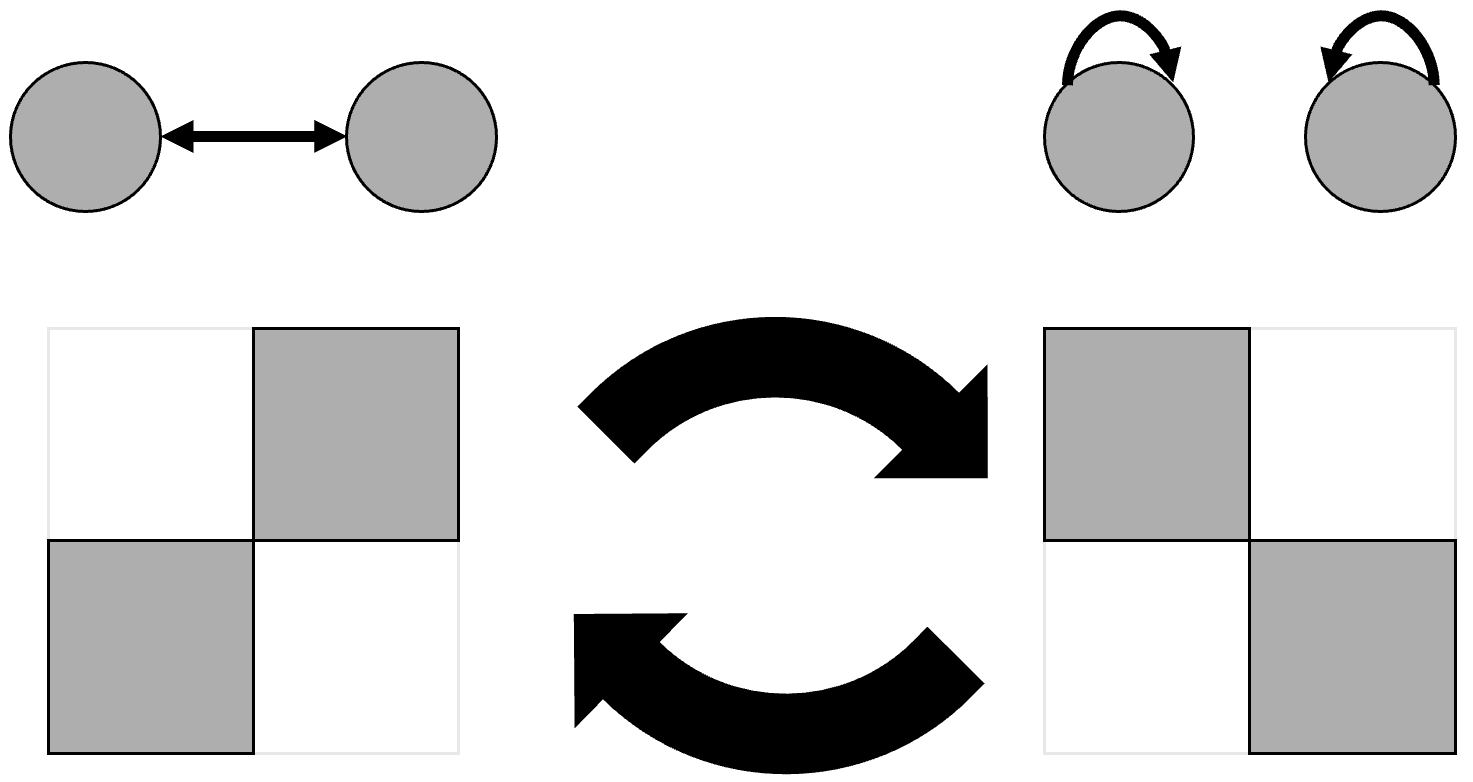
\includegraphics[scale= 0.24]{pictures/heatmap.png}
        \caption{Top: The given graph. Bottom: A heatmap of the corresponding adjacency matrix (gray: $a_{ij} = 1$, white: $a_{ij} = 0$)}
        \label{fig:non_convergence_heatmap}
\end{figure}
%     $\mat M = \begin{bmatrix}
% 0 & 1\\
% 1 & 0
% \end{bmatrix}$, if we now multiply this matrix with itself, we can observe that $\mat M^2 = \begin{bmatrix}
% 1 & 0\\
% 0 & 1
% \end{bmatrix}$ and then again \\ $\mat M^3 = \begin{bmatrix}
% 0 & 1\\
% 1 & 0
% \end{bmatrix}$
% \\
If the row-stochastic matrix $\mat M$, shown on the left in \cref{fig:non_convergence_heatmap}, is multiplied by itself, it takes the form shown on the left for uneven powers $\mat M^{2k+1}$, and the form on the right for even powers $\mat M^{2k}$. Therefore, $\lim_{k\rightarrow\infty}\mat M^k$ does not exist. The real-world counterpart for this example would be a pair of individuals who swap their two opinions at each revision.

Thus, we need to find necessary conditions for the convergence of row-stochastic matrices. Every square matrix $\mat A \in \CC^{n\times n}$ is similar to a block diagonal matrix $\mat J \in \CC^{n\times n}$, also called the Jordan normal form of $\mat A$, meaning $\mat A = \mat T \mat J \mat T^{-1}$ for an invertible matrix $\mat T \in \CC^{n\times n}$. The blocks on the diagonal of the Jordan matrix are called Jordan blocks $\mat{J_i}$ and have the form
\[\mat{J_i} = \begin{bmatrix}
\lambda_i & 1 & 0 & \dots & 0 \\
0 & \lambda_i & \ddots  & \ddots & \vdots \\
\vdots & \ddots & \ddots & 1 & 0 \\
0 & \ddots & 0 & \lambda_i & 1 \\
0 & 0 & \dots & 0 & \lambda_i
\end{bmatrix}\ , \]
% \[\mat{J} = \begin{bmatrix}
% \mat{J_i} &  & \makebox(0,0){\text{\huge0}} \\
% \makebox(0,0){\text{\huge0}} & \ddots & \\
%  & & \mat{J_i}
% \end{bmatrix}\ , \]
% \[\mat{J_i} = \begin{bmatrix}
% \lambda_i & 1 &  & \makebox(0,0){\text{\huge0}} \\
%  & \lambda_i & \ddots  &  \\
% \makebox(0,0){\text{\huge0}} &  & \ddots & 1 \\
%  &  &  & \lambda_i
% \end{bmatrix}\ , \]
where $\lambda_i$ is the $i$-th eigenvalue of $\mat A$. 

As $\mat A^k = \mat T \mat J^k \mat T^{-1}$, %begründen/zeigen mit TJT-1T,... (t-1 & t kürzen sich)
we can use this equation to find the limit of $\mat A^k$, as $\lim_{k\rightarrow\infty}\mat A^k = \mat T (\lim_{k\rightarrow\infty} \mat J^k) \mat T^{-1}$. Therefore, it suffices to show that $\mat J^k$ converges, to prove that $\mat A^k$ converges.

As the $k$-th power of a Jordan block $\mat{J_i} \in \CC^{l\times l}$ with the eigenvalue $\lambda_i$ has the form 
\[\mat{J_i}^k = \begin{bmatrix}
\lambda_i^k & \binom{k}{1}\lambda_i^{k-1} & \binom{k}{2}\lambda_i^{k-2} & \dots & \binom{k}{l-1}\lambda_i^{k-l+1}\\
0 & \lambda_i^k & \binom{k}{1}\lambda_i^{k-1} & \ddots & \vdots\\
\vdots & \ddots & \ddots & \ddots & \binom{k}{2}\lambda_i^{k-2}\\
0 & \ddots & 0 & \lambda_i^k & \binom{k}{1}\lambda_i^{k-1}\\
0 & 0 & \dots & 0 & \lambda_i^k
\end{bmatrix}\ , \] % ref bullo

% \[\mat{J_i}^k = \begin{bmatrix}
% \lambda_i^k & \binom{k}{1}\lambda_i^{k-1} & \binom{k}{2}\lambda_i^{k-2} & \dots & \binom{k}{l-1}\lambda_i^{k-l+1}\\
%  & \lambda_i^k & \binom{k}{1}\lambda_i^{k-1} & \ddots & \vdots\\
%  &  & \ddots & \ddots & \binom{k}{2}\lambda_i^{k-2}\\
%  & \makebox(0,0){\text{\huge0}} &  & \lambda_i^k & \binom{k}{1}\lambda_i^{k-1}\\
%  &  &  &  & \lambda_i^k
% \end{bmatrix}\ , \] % ref bullo
we can conclude the following conditions, shown in \cite{Bullo_lecture}, for the convergence of matrix $\mat A$. First, the magnitudes of all of its eigenvalues $\lambda_i$ must be $|\lambda_i| \leq 1$. If $|\lambda_i| > 1$, then all non-zero entries $(\mat{J_i})_{ij}$ of $\mat{J_i}$ diverge with $\lim_{k\rightarrow\infty}(\mat{J_i}^k)_{ij} = \infty$. When some Jordan block $\mat{J_i}$ diverges for $\lim_{k\rightarrow\infty}$, then trivially the Jordan matrix $\mat J$, and thus also $\mat A$, diverge as well.
Second, if $\lambda_j = -1$ is an eigenvalue of $\mat A$, then the entries $\lambda_j$ on the diagonal of the corresponding Jordan block $\mat{J_j}$ diverge for $\lim_{k\rightarrow\infty}\mat{J_j}^k$, as the powers $\lambda_j^k$ oscillate between $-1$ and $1$. Thus, $\mat A$ also oscillates, as can be observed in \cref{fig:non_convergence_heatmap}.
Third, if $\lambda_m = 1$ is an eigenvalue of $\mat A$, it needs to be semisimple, meaning that its geometric and algebraic multiplicities are equal. In other words, the corresponding Jordan blocks $\mat{J_m}$ must have size $1$, i.e., $\mat{J_m} = [\lambda_m]$.
If this condition is not satisfied, the entries $(\mat{J_m})_{ij}$ with $j>i$ diverge for $\lim_{k\rightarrow\infty}(\mat{J_m}^k)_{ij} = \infty$. In the following, we will refer to the eigenvalue 1 of $\mat A$, also called the dominant eigenvalue, as $\lambda_1$.

Additionally, because $\mat T$ is invertible, we know that $\mat T,\mat T^{-1}\neq \zerosmatr$. Therefore, if $\mat A$ has the semisimple eigenvalue $\lambda_1$ and the limit of $\mat A$ exists, then 
\[\lim_{k\rightarrow\infty}\mat{A}^k = \mat T(\lim_{k\rightarrow\infty}\mat{J}^k)\mat T^{-1} \neq \zerosmatr \ ,\] 
as the Jordan blocks corresponding to $\lambda_1$ converge against $\lim_{k\rightarrow\infty}{\mat{J_1}^k} = \lim_{k\rightarrow\infty}{[1]^k} = [1]$, i.e., $\lim_{k\rightarrow\infty}\mat J^k \neq \zerosmatr$. We refer to such a matrix $\mat A$ as semi-convergent.
% On the contrary, if $\mat A$ has no eigenvalue $\lambda_1$, then $\lim_{k\rightarrow\infty}\mat A^k = \lim_{k\rightarrow\infty}\mat J^k = \zerosmatr$ and is referred to as convergent.

Because $\mat A$ is row-stochastic, by definition
\begin{equation}\label{eq:1_eigenvalue_all_row_stochastic_mat}
    \mat A\ones= \ones = 1\cdot\ones, \textnormal{with } \ones \neq \zeros\ ,
\end{equation}
as all rows have unit sum. Thus, $\lambda_1$ is an eigenvalue of all matrices $\mat A$ of the model which are consequently semi-convergent, if a limit exists.

% if 1 not eigenvalue then convergent
We can summarize these findings in the following \cref{th:semi_conv}, found in \cite{Bullo_lecture}.
\begin{theorem}\label{th:semi_conv}
    A row-stochastic matrix $\mat A$ is semi-convergent (i.e., $\lim_{k\rightarrow\infty}\mat A^k \neq \zerosmatr$ exists) if and only if:
    \begin{enumerate}[label=(\roman*)]
        \item 1 is an eigenvalue
        \item 1 a semisimple eigenvalue, and
        \item all other eigenvalues have magnitude less than 1. 
    \end{enumerate}
\end{theorem}
As shown, condition (i) of \cref{th:semi_conv} holds for all row-stochastic matrices. We will discuss under which circumstances the other conditions hold in the following section.

% \begin{lemma}\label{spectral_radius}
%     The set of all eigenvalues of a row-stochastic matrix A is a subset of the unit disk.
% \end{lemma}
% It follows from Lemma \ref{spectral_radius} that for all eigenvalues $\mu$ of a row-stochastic matrix A, $1 \geq |\mu| \geq 0$.

\subsubsection{Reaching a Consensus} \label{sec:reaching_consensus}
To now determine when a consensus is reached,  we will utilize the Perron-Frobenius \cref{th:perron-frobenius}, namely, irreducible and primitive matrices.
\begin{definition} [Irreducible and primitive matrices] \label{def:irr_prim_mat}
    For $n \geq 2$, a non-negative matrix $\mat A \in \RR_{\geq0}^{n\times n}$ is 
    \begin{enumerate}[label=(\roman*)]
        \item \textit{irreducible} if $\sum_{k=0}^{n-1}\mat A^k > 0$
        \item \textit{primitive} if there exists a $k \in \NN$, such that $\mat A^k >0$.
    \end{enumerate}
\end{definition}
Moreover, a primitive matrix is necessarily also irreducible, see \cite{Bullo_lecture}.

When applying the Perron-Frobenius Theorem to row-stochastic matrices $\mat A$, we get the following, as found in \cite{Bullo_lecture}.
\begin{theorem}[Perron-Frobenius Theorem]\label{th:perron-frobenius}
    Let the row-stochastic $\mat A \in [0,1]^{n\times n}$ with $n\geq 2$, then if $\mat A$ is irreducible,
    \begin{enumerate}[label=(\roman*)]
        \item the eigenvalue $\lambda_1$ is simple.
    
    \textnormal{If additionally $\mat A$ is primitive, then}
        \item the eigenvalue $\lambda_1$ satisfies $\lambda_1 > |\lambda_i|$ for all other eigenvalues $\lambda_i$ of $\mat A$. 
    \end{enumerate}
\end{theorem}
Therefore, according to the Perron-Frobenius \cref{th:perron-frobenius}, if $\mat A$ is irreducible and row-stochastic, then $\lambda_1$ is simple, which is a sufficient condition for semisimple, thus fulfilling condition (ii) of \cref{th:semi_conv}. Moreover, if additionally $\mat A$ is primitive, then all eigenvalues $\lambda_i \neq 1$ have magnitude less than 1, i.e., $\lambda_1 > |\lambda_i|$, thus satisfying condition (iii) of \cref{th:semi_conv}.
It can therefore be concluded that if a row-stochastic matrix is primitive, then $\mat A$ is semi-convergent, i.e., the model converges.

However, it can often be computationally expensive to check whether a given matrix is irreducible or primitive. Therefore, we will now relate these conditions to graph properties, which are typically easier to verify.

We can translate any instance of the DeGroot model into a digraph $\gG=(V,E)$ with the nodes $V(\gG) = \{1, \dots,n\}$ representing the individuals and the edges $E(\gG) = \{(i,j)|a_{ij} > 0\}$ with the corresponding weighted adjacency matrix $\mat A$, defined in \cref{sec:degroot}. We can now observe that a path of length $k$ exists from node $i$ to node $j$ in $\gG$ if and only if for the $k$-th power of the adjacency matrix, $(\mat A^k)_{ij} > 0$. For this, we offer an independent proof.

\begin{proof}
    Let $\mat A\in[0,1]^{n\times n}$. There trivially exists a path of length $1$ from node $i$ to node $j$, precisely when $(\mat A)_{ij}=a_{ij}>0$, i.e., there exists an edge from $i$ to $j$. Assume that the observation is correct for any $k\in \underline{n}$. If there exists a path of length $k+1$ from $i$ to $j$, then there exists a path of length $k$ from $i$ to some node $l\in\underline{n}$ with $(l,j)\in E(\gG)$, i.e., $(\mat A)_{lj}>0$. As $(\mat A^{k+1})_{ij} = (\mat A^k\cdot \mat A)_{ij} = \sum_{m=1}^{n}(\mat A^k)_{im}\cdot (\mat A)_{mj} \geq (\mat A^k)_{il}\cdot (\mat A)_{lj}>0$, because by the induction hypothesis $(\mat A^k)_{il}>0$. In the other direction, if $(\mat A^{k+1})_{ij}>0$, then there must be at least one $l\in \underline{n}$, such that $(\mat A^k)_{il}\cdot (\mat A)_{lj} >0$. Thus, using the induction hypothesis, there must exist a path of length $k$ from $i$ to $l$ and $(l,j)\in E(\gG)$. Therefore, there exists a path of length $k+1$ from $i$ to $j$ over $l$.
\end{proof}

This means that our digraph $\gG$ is strongly connected, if and only if for every pair of nodes $(i,j)$ with $i\neq j$, $(\mat A^k)_{ij}>0$, for a $k<n$. It trivially suffices to ensure this property for $k<n$, as if a path of length $k\geq n$ exists, then at least $n+1$ nodes are visited, i.e., at least one node is visited multiple times. Consequently, a loop exists in this path which can be removed, resulting in a path of length $k<n$. Thus, $\gG$ is strongly connected if and only if $\sum_{k=0}^{n-1}\mat A^k > 0$, i.e., $\mat A$ is irreducible, see \cref{def:irr_prim_mat}. Moreover, as shown in \cite{Bullo_lecture}, the weighted adjacency matrix $\mat A$ is primitive if and only if $\gG$ is strongly connected and aperiodic. Thus, these two properties ensure the asymptotic convergence of the model.

% Now we can examine, when the model reaches consensus.
% \begin{theorem}\label{th:consensus}
%     Let A be a row-stochastic matrix, then the two following statements are equivalent:
%     \begin{enumerate}[label=(\roman*)]
%         \item the eigenvalue 1 is simple and all other eigenvalues $\mu$ satisfy $1 >\mu$.
%         \item A is semi-convergent and $\lim_{k\rightarrow\infty}A^k = \ones w^\T$, where $w\in \RR^n$ satisfies $w \geq 0$, $\ones^\T w = 1$, and $w^\T A = w$
%     \end{enumerate}
%     (If one of these conditions is satisfied (meaning both are satisfied), then the solution of our model $P^k = A^kP$ with $k \rightarrow \infty$ satisfies $\lim_{k\rightarrow\infty}P^k = (w^\T P)\ones$) %Only write: then consensus reached (equation moved to 2.1.2)
% \end{theorem}

Now, we can examine when the model reaches consensus. As stated above, all eigenvalues of a row-stochastic matrix $\mat A$ must have a magnitude less than 1, except for the eigenvalue $\lambda_1$, for $\mat A^k$ to converge. Moreover, the eigenvalue $\lambda_1$ needs to be semisimple, for the corresponding Jordan blocks to converge.
Therefore, if we let $m_g \in \underline{n}$ denote the geometric multiplicity (and thus also the algebraic multiplicity) of eigenvalue $\lambda_1$, then the limit of the Jordan matrix $\lim_{k\rightarrow\infty}\mat J^k$ is a diagonal matrix with a 1 in $m_g$ entries of the diagonal.
Let $\vec{c_1},\dots,\vec{c_{m_g}}$ denote the columns of $\mat T$ and $\vec{r_1}^\T,\dots,\vec{r_{m_g}}^{\T}$ denote the rows of $\mat T^{-1}$ that correspond to the Jordan blocks for the eigenvalue $\lambda_1$. Moreover, let $(c_{i})_j$ and $(r_{i})_j$ denote the $jth$ entry of these vectors. Then

\begin{multline} \label{eq:col_row_A^k}
    % \lim_{k\rightarrow\infty}\mat A^k 
    % \mat{A^{fin}} =
    \mat T(\lim_{k\rightarrow\infty}\mat J^k)\mat T^{-1} = \begin{bmatrix}
        \vec{c_{1}} & \dots & \vec{c_{{m_g}}}
    \end{bmatrix}\cdot
    \begin{bmatrix}
        \vec{r_{1}} & \dots & \vec{r_{{m_g}}}
    \end{bmatrix}^{\T}\\
    = \begin{bmatrix}
        (c_{1})_1& \dots & (c_{{m_g}})_1\\
        \vdots & \vdots & \vdots\\
        (c_{1})_n & \dots & (c_{{m_g}})_n
    \end{bmatrix}\cdot
    \begin{bmatrix}
        (r_{1})_1 & \dots & (r_{1})_n\\
        \vdots & \vdots & \vdots\\
        (r_{{m_g}})_1 & \dots & (r_{{m_g}})_n
    \end{bmatrix}
\end{multline}

% \begin{multline}
%     \mat A^k = \mat T\mat J^k\mat T^{-1} =\\ \begin{bmatrix}
%         c_{11}r_{11}+\dots +c_{{m_g}1}r_{{m_g}1} & \dots & c_{11}r_{1n}+\dots + c_{{m_g}1}r_{{m_g}n}\\
%         \vdots & \vdots & \vdots\\
%         c_{1n}r_{11}+\dots +c_{{m_g}n}r_{{m_g}1} & \dots & c_{1n}r_{1n}+\dots +c_{{m_g}n}r_{{m_g}n}
%     \end{bmatrix}
% \end{multline}

To reach an asymptotic consensus, all rows of $\mat{A^{fin}}$ must be equal. Thus, all columns $\vec{c_1}, \dots, \vec{c_{m_g}}$ of $\mat T$ need to be equal, see \cref{eq:col_row_A^k}.

As, $\mat A = \mat T\mat J\mat T^{-1} \iff \mat A\mat T = \mat T\mat J \iff \mat T^{-1}\mat A = \mat J\mat T^{-1}$, if $\lambda_1$ is semisimple, then $\mat A\vec{c_i} = \lambda_1\vec{c_i}$ and $\vec{r_i}\mat A = \lambda_1\vec{r_i}$, i.e., $\vec{c_i}$ is the right eigenvector and $\vec{r_i}^\T$ the left eigenvector of $\lambda_1$, as shown in \cite{Bullo_lecture}. Because the number of dimensions of an eigenspace is equal to the geometric multiplicity of the corresponding eigenvalue, the eigenspace of $\lambda_1$ has $m_g$ dimensions \cite{axler}.
Thus, all of the $m_g$ eigenvectors $c_i$ of $\lambda_1$ need to be linearly independent. Therefore, they cannot be equal if the geometric multiplicity $m_g>1$, meaning the rows of $\mat{A^{fin}}$ are equal if and only if $m_g = 1$, i.e., $\lambda_1$ is simple.

Thus, the model reaches an asymptotic consensus if and only if the row-stochastic matrix $\mat A$ is semi-convergent and $\lambda_1$ is simple. Therefore, according to the Perron-Frobenius \cref{th:perron-frobenius}, the model converges when $\mat A$ is primitive. However, $\mat A$ being primitive is not a necessary condition to reach an asymptotic consensus. Intuitively, as all final opinion values depend on the individual $i$ corresponding to the simple eigenvalue $\lambda_1$, all other individuals must be connected to this individual $i$. Otherwise, their opinion value could not be influenced by individual $i$. Thus, the node corresponding to individual $i$ needs to be globally reachable, i.e., reachable from all other nodes. In other words, there must exist a globally reachable node, which corresponds precisely to $\lambda_1$, for the model to asymptotically reach a consensus. This condition is sufficient to determine whether asymptotic consensus is reached, see \cite{Bullo_lecture}.

% \begin{multline}
%     \mat A^k = \mat T\mat J^k\mat T^{-1} = \\ \begin{bmatrix}
%         c_{11}r_{11}+c_{21}r_{21}+\dots c_{{m_g}1}r_{{m_g}1} & \dots & c_{11}r_{1n}+\dots + c_{{m_g}1}r_{{m_g}n}\\
%         \vdots & \vdots & \vdots\\
%         c_{1n}r_{11}+c_{2n}r_{21}+\dots c_{{m_g}n}r_{{m_g}1} & \dots & c_{1n}r_{1n}+\dots +c_{{m_g}n}r_{{m_g}n}
%     \end{bmatrix}
% \end{multline}



\subsubsection{Calculating the Consensus}\label{sec:calculating_conv}
However, we are interested not only in when a consensus is reached, but also in what consensus is reached. Therefore, we will take a look at how the consensus can be calculated in case it is reached.

% \begin{theorem}\label{th:consensus_value}
%     Let A be a non-negative matrix. Assume that the dominant eigenvalue $\lambda$ is simple and strictly larger in magnitude, than all other eigenvalues. Then $\frac{A}{\lambda}$ is semi-convergent and 
%     \begin{equation}
%         \lim_{k\rightarrow\infty}\frac{A^k}{\lambda^k}= vw^\T \ ,
%     \end{equation}
%     where $v$ and $w$ are the right and left dominant eigenvectors of A normalized so that $v \geq0$, $w \geq0$ and $v^\T w$
% \end{theorem}
As we concluded in \cref{sec:reaching_consensus}, the model converges to a consensus if and only if $\mat A$ is semi-convergent and $\lambda_1$ is simple. Thus, using \cref{eq:col_row_A^k}, $\lim_{k\rightarrow\infty}\mat A^k = \vec c \cdot\vec r$, where $\vec c = [c_1, \dots, c_n]^\T$ and $\vec r = [r_1, \dots, r_n]$ are the right and left eigenvectors of $\lambda_1$.
 
Because $\ones$ is an eigenvector of every row-stochastic matrix, as shown in \cref{eq:1_eigenvalue_all_row_stochastic_mat}, the right eigenvector $\vec{c}$ can be chosen as $\vec c = \ones$. Then
\begin{equation}\label{eq:limit_A}
    \lim_{k\rightarrow\infty}\mat A^k= \ones \vec r = 
    \begin{bmatrix}
        \vec r\\
        \vdots\\
        \vec r
    \end{bmatrix}_{n\times n} = 
    \begin{bmatrix}
         r_1 & \dots &  r_n\\
        \vdots & \vdots & \vdots\\
         r_1 & \dots &  r_n
    \end{bmatrix}\ .
\end{equation}
To calculate the consensus, we now need to combine \cref{eq:limit_A} with \cref{eq:iteration}, such that
\begin{equation}\label{eq:limit_P}
    \vec{p^{fin}} = \lim_{k\rightarrow\infty}\vec p^k = (\lim_{k\rightarrow\infty}\mat A^k)\vec{p_0} = 
    \begin{bmatrix}
        \vec r\\
        \vdots\\
        \vec r
    \end{bmatrix}_{n\times n}
    \begin{bmatrix}
        v_1\\
        \vdots\\
        v_n
    \end{bmatrix}\ .
\end{equation}
Therefore, the consensus is equal to 
\[v^{fin}_i = r_1v_1+r_2v_2+\dots +r_nv_n \ ,\]
for all $i \in \underline{n}$.

In summary, only the left eigenvector $\vec{r}$ of $\lambda_1$ of the matrix $\mat{A}$ is required, in addition to the vector of the initial opinion values $\vec{p_0}$, to calculate the final opinion values.

Moreover, we can interpret the structure of this left eigenvector $\vec{r}^\T$ as a weighted average over the initial opinion values in $\vec{p_0}$. The weights intuitively depend on the centrality of the corresponding node, i.e., how many other nodes are connected to it. Thus, if, for example, a given instance of the model is not strongly connected but has one sink component (see \cref{sec:prelim_notation}), then only the weights corresponding to nodes in the sink are non-zero.

\subsubsection{Measuring the Speed of Convergence}\label{sec:speed_convergence}
Finally, after analyzing when and what consensus is reached, we will examine whether we can measure the speed of convergence, i.e., how long it takes for the group to asymptotically reach a consensus.

Rather intuitively, we can observe that the speed of convergence depends on the eigenvalues of matrix $\mat A$. As we have shown in \cref{sec:when_convergence}, the convergence of A can be represented by its Jordan matrix, as $\mat A^k = \mat T\mat J^k\mat T^{-1}$. The matrix $\mat J^k$ converges when all eigenvalues $|\lambda_i| < 1$, i.e., all eigenvalues except $\lambda_1$, have converged against $0$, with $\lim_{k\rightarrow\infty}\lambda_i^k = 0$. Therefore, the speed of convergence depends on the size of the eigenvalues of $\mat A$. More specifically, the convergence rate is dependent on the largest eigenvalue $\lambda_{max}$, with $|\lambda_{max}| \geq |\lambda_i|$ for all $i \in \{2,\dots,n\}$.

For this $\lambda_{max}$, it trivially holds that $\lambda_{max}^k \geq \lambda_i^k$, with $k > 0$, for all $i\in \{2,\dots,n\}$.
Therefore, we can define the upper bound 
\[|v_{ik} - \vec r \vec{p_0}| = |v_{ik} - v^{fin}_i| = O(\lambda_{max}^k)\ ,\]
as in \cite{DeMarzo}.
This bound describes that the distance between all opinion values in revision $k$ and the final opinion value depends on the size of the eigenvalue $\lambda_{max}$.
Thus, we know for all pairs of semi-convergent, row-stochastic matrices $\mat A$ and $\mat{A^{'}}$, that if $\lambda_{max} < \lambda_{max}^{'}$, then $\lim_{k\rightarrow\infty}\mat A^k$ converges faster asymptotically than $\lim_{k\rightarrow\infty}(\mat{A^{'}})^k$. 
This can be observed in \cref{fig:convergence_speed_quick} and \cref{fig:convergence_speed_low}. The eigenvalue $\lambda_{max}$ of the adjacency matrix used in \cref{fig:convergence_speed_low} is much smaller in magnitude than the one of the adjacency matrix used in \cref{fig:convergence_speed_quick}. Thus, the model in \cref{fig:convergence_speed_low} converges faster asymptotically, than the model in \cref{fig:convergence_speed_quick}, as can be seen in the figures.

Therefore, we can measure the convergence rate of an instance of the model by calculating the difference between $\lambda_1 - |\lambda_{max}|$. This eigengap between the dominant eigenvalue $\lambda_1$ and $\lambda_{max}$ is also referred to as the spectral gap. 
% Because of its relevance, this eigenvalue is often called the Fiedler eigenvalue in other literature.

% \[\begin{bmatrix}
%         \vec r\\
%         \vdots\\
%         \vec r
% \end{bmatrix}\]

% \begin{tikzpicture}[
%     node distance=.5cm,
%     vertex/.style={circle,draw,minimum size=6mm,font=\small},
%     >=Stealth,
%     every edge quotes/.style={font=\scriptsize,fill=white,inner sep=2pt}
% ]
% % Define nodes (vertices 0-7)
% \node[vertex] (0) at (90:2cm) {0};
% \node[vertex] (1) at (45:2cm) {1};
% \node[vertex] (2) at (0:2cm) {2};
% \node[vertex] (3) at (-45:2cm) {3};
% \node[vertex] (4) at (-90:2cm) {4};
% \node[vertex] (5) at (-135:2cm) {5};
% \node[vertex] (6) at (180:2cm) {6};
% \node[vertex] (7) at (135:2cm) {7};

% % Draw edges with weights
% \draw[->] (0) edge[bend right=15,"0.3"] (1);
% \draw[->] (1) edge[bend right=15,"1"] (0);
% \draw[->] (0) edge["0.7"] (2);
% \draw[->] (2) edge["0.5"] (4);
% \draw[->] (2) edge["0.5"] (5);
% \draw[->] (3) edge["1"] (4);
% \draw[->] (4) edge["1" '] (1);
% \draw[->] (5) edge["1"] (7);
% \draw[->] (6) edge["0.45"] (3);
% \draw[->] (6) edge["0.55" '] (4);
% \draw[->] (7) edge["1" '] (6);

% \end{tikzpicture}

\begin{table}[H]
\caption{Adjacency matrix used in \cref{fig:convergence_speed_quick} with $|\lambda_{max}| \approx 0.932$. A darker square corresponds to an entry with a larger relative value.}
\label{tb:heatmap_low}
\centering
\pgfplotstabletypeset[
    color cells,
    create on use/rownum/.style={
        create col/expr=\pgfplotstablerow+1
    },
    columns/rownum/.style={column name= , column type=r},
    columns/0/.style={column name=1},
    columns/1/.style={column name=2},
    columns/2/.style={column name=3},
    columns/3/.style={column name=4},
    columns/4/.style={column name=5},
    columns/5/.style={column name=6},
    columns/6/.style={column name=7},
    columns/7/.style={column name=8}
]
{
10, 30, 69, 0, 0, 0, 0, 0
99, 10, 0, 0, 0, 0, 0, 0
0, 0, 10, 0, 0, 99, 0, 0
0, 0, 0, 10, 99, 0, 0, 0
0, 99, 0, 0, 10, 0, 0, 0
0, 0, 0, 0, 0, 10, 0, 99
0, 0, 0, 45, 54, 0, 10, 0
0, 0, 0, 0, 0, 0, 99, 10
}
\end{table}


% \[\begin{bmatrix}
% d_1 & 0  &\dots & 0\\
% 0 & d_2 & \ddots & \vdots\\
% \vdots & \ddots & \ddots & 0\\
% 0 & \dots & 0 & d_n
% \end{bmatrix}.\]

\begin{figure}[H]
    \centering
        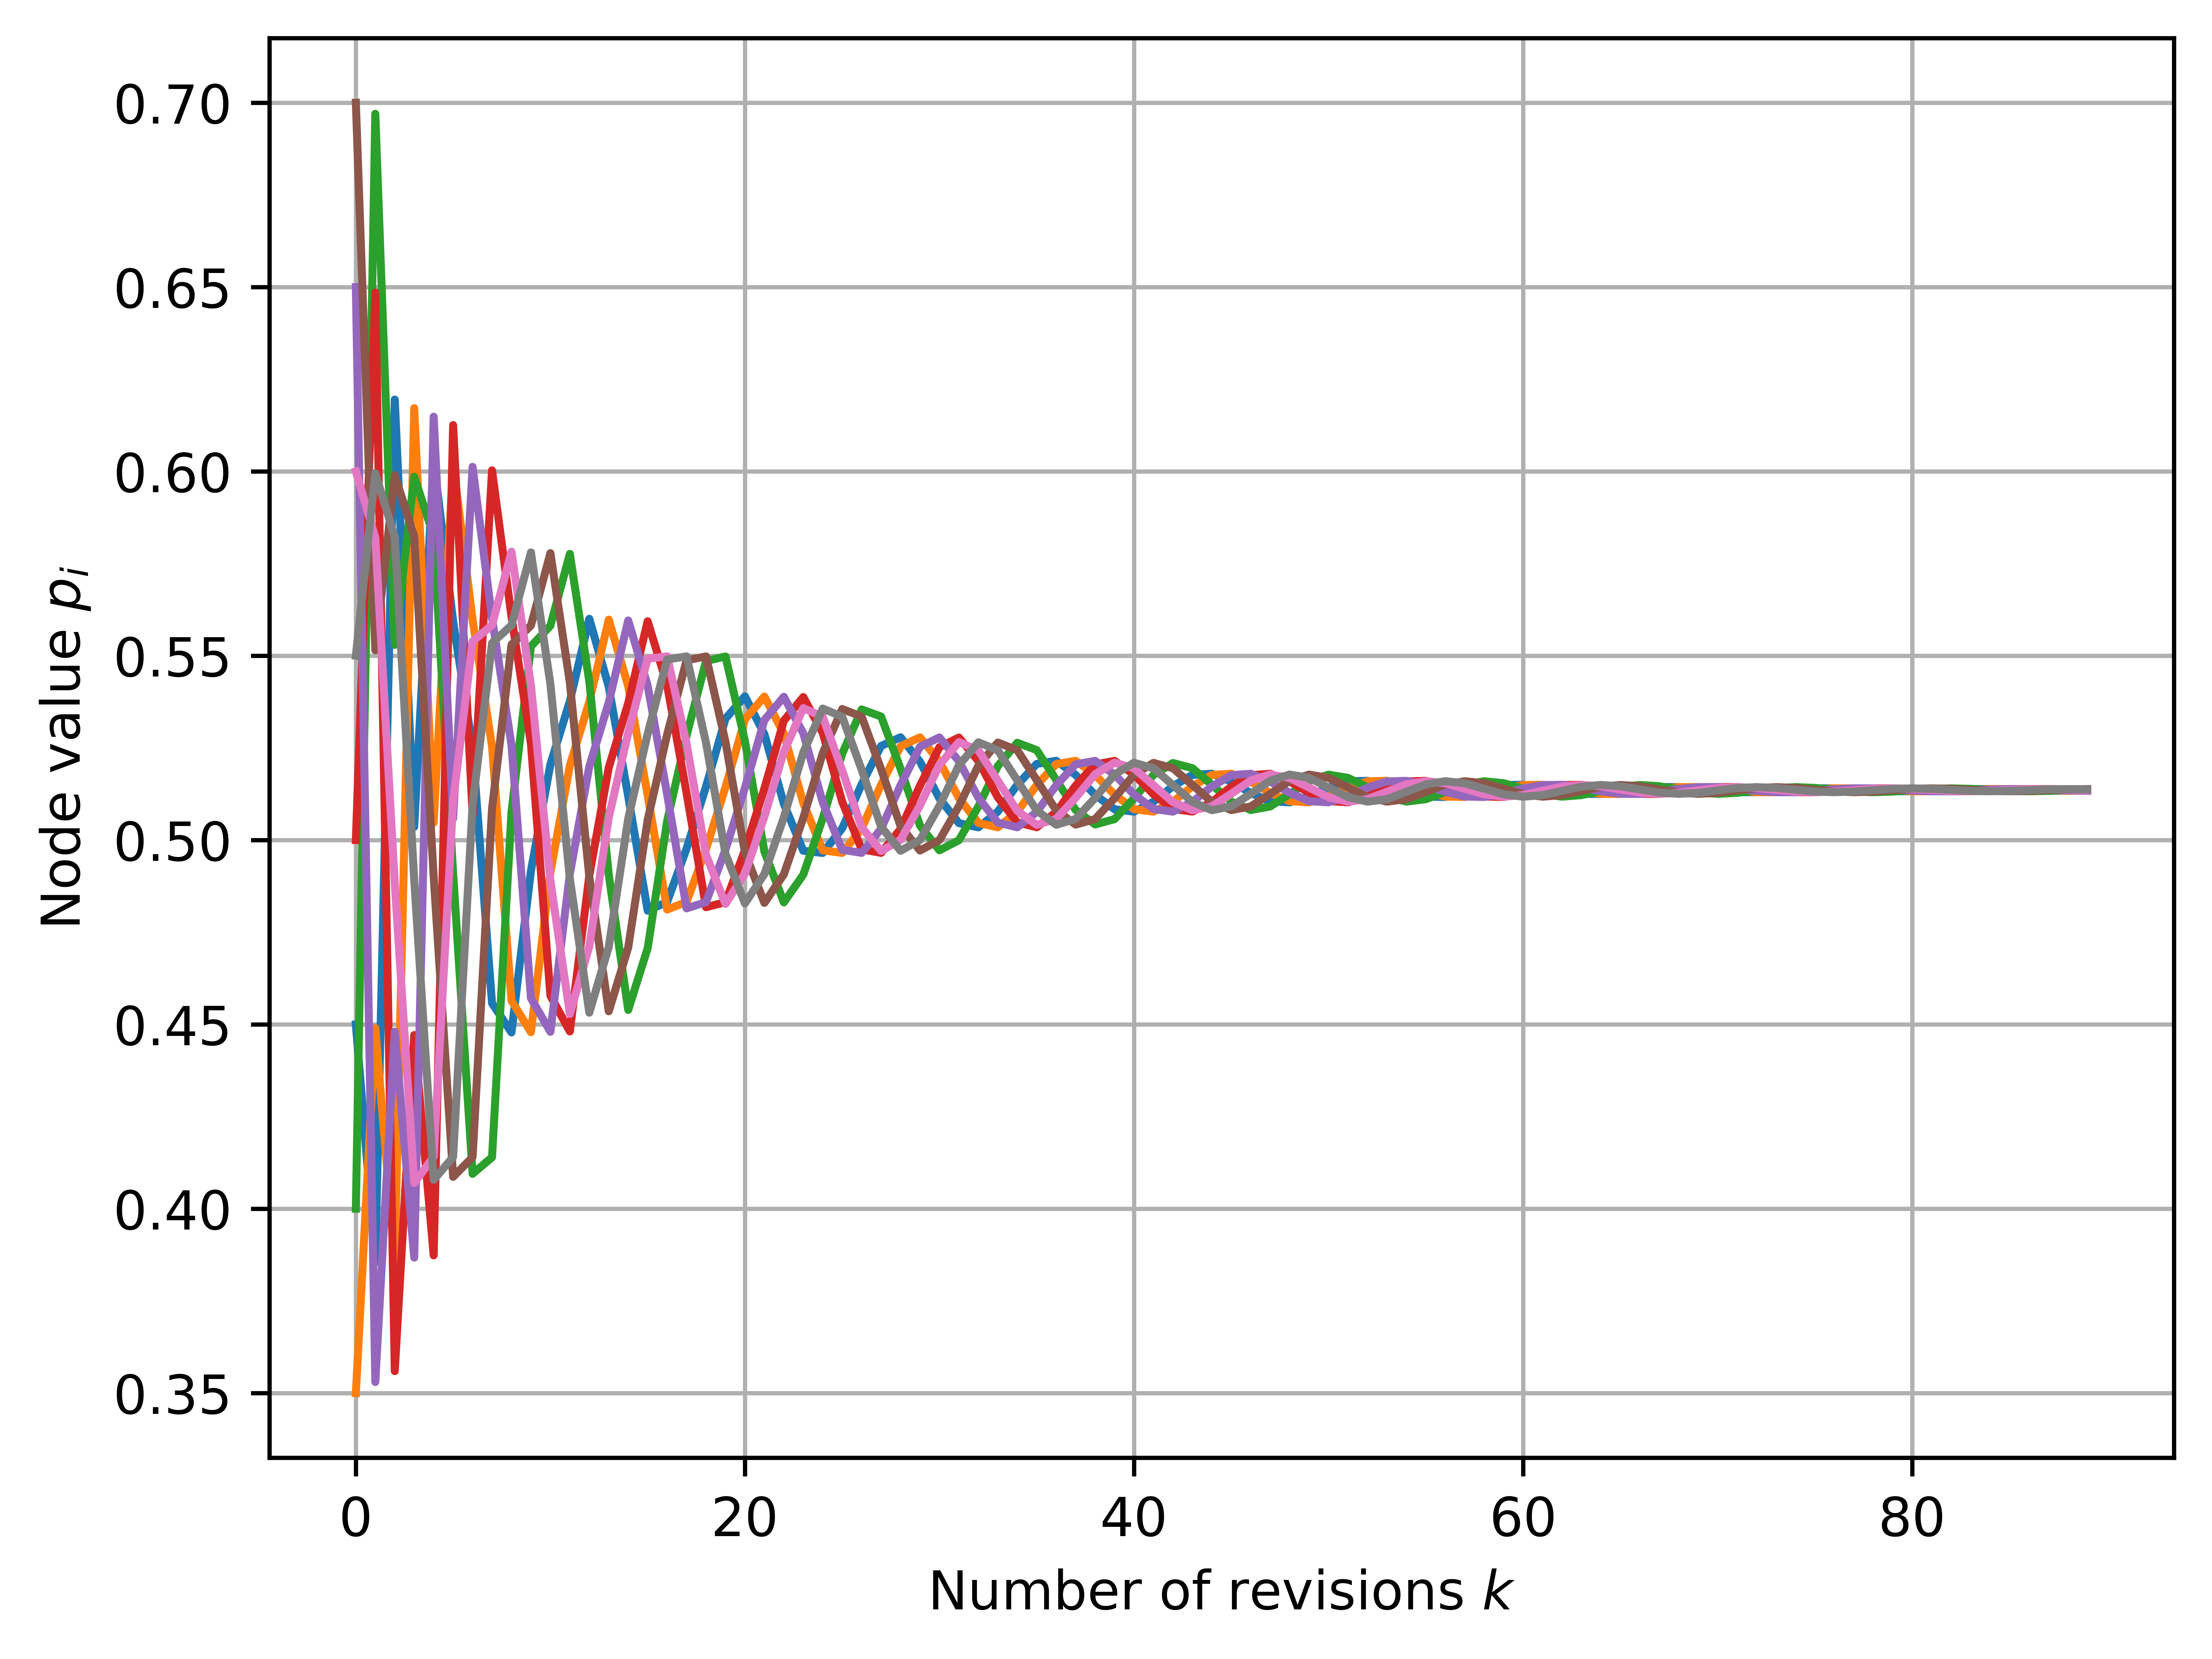
\includegraphics[scale= 0.5]{pictures/convergence_low.png}
        \caption{The convergence towards a consensus for an instance of the DeGroot model with the adjacency matrix shown in \cref{tb:heatmap_low}.}
        \label{fig:convergence_speed_quick}
\end{figure}

\begin{table}[H]\caption{Adjacency matrix used in \cref{fig:convergence_speed_low} with $|\lambda_{max}| \approx 0.449$. A darker square corresponds to an entry with a larger relative value.}\label{tb:heatmap_high}
\centering
\pgfplotstabletypeset[
    color cells,
    create on use/rownum/.style={
        create col/expr=\pgfplotstablerow+1
    },
    columns/rownum/.style={column name= , column type=r},
    columns/0/.style={column name=1},
    columns/1/.style={column name=2},
    columns/2/.style={column name=3},
    columns/3/.style={column name=4},
    columns/4/.style={column name=5},
    columns/5/.style={column name=6},
    columns/6/.style={column name=7},
    columns/7/.style={column name=8}
]{
25, 0, 0, 12.5, 12.5, 25, 25, 0
0, 25, 50, 0, 0, 0, 25, 0
25, 0, 12.5, 0, 50, 12.5, 0, 0
50, 0, 0, 12.5, 25, 0, 0, 12.5
0, 50, 0, 0, 12.5, 0, 25, 12.5
0, 0, 0, 50, 25, 12.5, 0, 12.5
0, 25, 0, 50, 0, 0, 25, 0
25, 0, 0, 0, 50, 0, 12.5, 12.5
}
\end{table}

\begin{figure}[H]
    \centering
        \includegraphics[scale= 0.4]{pictures/convergence_high.png}
        \caption{The convergence towards a consensus for an instance of the DeGroot model with the adjacency matrix shown in \cref{tb:heatmap_high}.}
        \label{fig:convergence_speed_low}
\end{figure}

\subsection{Influence of Network Properties on the Convergence}\label{sec:network_prop}
As shown in \cref{sec:reaching_consensus}, we can represent the DeGroot model as a digraph $\gG$ with the individuals as nodes and $\mat A$ as the weighted adjacency matrix. Therefore, we will look at how certain network and graph properties can influence the model.

First, we will look at graphs $\gG$ that consist of multiple strongly connected subgraphs $\gG_i$, i.e., $\gG_i(E) \subset \gG(E)$ and $\gG_i(V) \subset \gG(V)$.
As concluded in an observation in \cref{sec:reaching_consensus}, the model reaches a consensus if and only if a globally reachable node exists. Thus, no consensus is reached for these graphs $\gG$, as such a node cannot exist by definition. 

However, according to \cite{Bullo_lecture}, the eigenvalue $\lambda_1$ is semisimple with the geometric multiplicity $m_g$ and $|\lambda_j| < 1$ for all $j \in \{2,\dots,n\}$ if and only if $\gG$ has sinks $\gS_i$ (see \cref{sec:prelim_notation}) with $i\in\underline{m_g}$, that are all aperiodic. Such graphs $\gG$, that fulfill these conditions, therefore, have semi-convergent adjacency matrices $\mat A$, see \cref{th:semi_conv}.
Moreover, these graphs reach disagreement, instead of consensus, meaning that at least one pair of final opinion values $v_{i}^{fin} \neq v_{j}^{fin}$.
When calculating the final opinion values, as in \cite{Bullo_lecture}, we need to differentiate between strongly connected subgraphs and sinks. As the sinks $\gS_i$ have no outgoing edges, the final opinion values of the individuals in the sinks are not dependent on other individuals outside of their sink. Therefore, the final opinion value for nodes $j\in \gS_i$, with $i\in \underline{m_g}$, can be calculated as
\[v_j^{fin} = \vec{r_i} \vec{p_0}\ ,\]
where $\vec{r_i}$ is the corresponding left eigenvector, as in \cref{eq:limit_P}. However, the final opinion values of nodes in strongly connected subgraphs that are not sinks, i.e., that have outgoing edges to other strongly connected subgraphs, are dependent on nodes outside of their subgraph. Therefore, the final opinion value for nodes $j\notin \gS_i$, with $i\in \underline{m_g}$, is equal to
\[v_j^{fin} = \sum_{p=1}^{m_g}z_{ji}(\vec{r_i} \vec{p_0})\ ,\]
where $\vec{r_i}$ is the corresponding left eigenvector of the sink to which $j$ is connected. The $z_{ji}$, with $i\in \underline{m_g}$, are convex combination coefficients that are $z_{ji} > 0$ if and only if there exists a directed path from node $j$ to sink $i$.

Second, we will discuss how the connectedness of the graph can influence the convergence rate of the model. The conductance $\Phi$ of a graph $\gG$ is a measure to determine how connected a graph is. Similarly to \cite{lovasz1993random}, the measure can be defined for a set $S$ of nodes as
\[\Phi(S) = \frac{\sum_{i\in S,j\notin S}a_{ij}}{min(|S|,|V(\gG)\backslash S|)}\ .\]
The numerator $\sum_{i\in S,j\notin S}a_{ij}$ is the sum of the weights of the edges from $S$ to $V(\gG)\backslash S$, i.e., it describes how much combined weight the nodes in $S$ give to those in $V(\gG)\backslash S$. Therefore, the conductance of a set of nodes $S$ measures the connectedness of $S$ and $V(\gG)\backslash S$ compared to how connected the sets are themselves. For a graph $\gG$, its conductance is defined as $\Phi(\gG) = \min_{S\subset V(\gG)}\Phi(S)$. Thus, if the conductance of a graph $\gG$ is low, there exists a partition of the nodes into two sets ($S$ and $V(\gG)\backslash S$), such that the nodes $i,j \in S$ or $i,j \notin S$ are highly connected, while nodes $i\in S,\ j\notin  S$ are only sparsely connected. However, if the conductance of the graph $\gG$ is large, then the entirety of $\gG$ is highly connected. As shown in \cite{lovasz1993random}, this measure of conductance can be used to find the upper and lower bounds
\[\frac{\Phi(\gG)^2}{8}\leq 1-\lambda_{max} \leq \Phi(\gG)\ ,\]
for the eigenvalue $\lambda_{max}$. These bounds imply that a higher conductance, i.e., connectedness, of the graph results in a larger spectral gap and therefore in a smaller eigenvalue $\lambda_{max}$. Because we observed that $\lambda_{max}$ is an upper bound for the convergence rate of the model (see \cref{sec:speed_convergence}), we can conclude that highly connected graphs tend to converge faster than sparsely connected ones. This correlation can be observed in \cref{fig:convergence_speed_quick} and \cref{fig:convergence_speed_low}.

% \todo{(Weight-balanced $\rightarrow$ average consensus)}Lastly, we \dots weight-balanced graphs. \dots

% \begin{definition}[Periodic/Aperiodic graphs] %Def von wo anders? --> andere quelle
%     A strongly connected graph is called \textit{periodic}, if there exists a $k \in \NN_{>1}$, that divides the length of every simple cycle of the graph. A simple cycle refers to every possible path from any node $v$ back to itself.
% \end{definition}

% \begin{lemma}
%     Let $\gG$ be a weighted digraph and a be its corresponding adjacency matrix $\mat A$. Then any entry (i,j) of $\mat A^k$ is positive if and only if there exists a walk of length k from node i to node j in $\gG$.
% \end{lemma}

% Self-loops

% \begin{theorem}
%     Let $\gG$ be a weighted digraph with $n \geq 2$ nodes and with the corresponding weighted adjacency matrix $\mat A$. Then the following statements are equivalent:
%     \begin{enumerate}[label=(\roman*)]
%         \item $\mat A$ is irreducible
%         \item $\gG$ is strongly connected
%     \end{enumerate}
% \end{theorem}

% \begin{theorem}
%     Let $\gG$ be a weighted digraph with $n \geq 2$ nodes and with the corresponding weighted adjacency matrix $\mat A$. Then the following statements are equivalent:
%     \begin{enumerate}[label=(\roman*)]
%         \item $\mat A^{n-1}$ is positive, i.e., $\mat A$ is primitive 
%         \item $\gG$ is strongly connected
%     \end{enumerate}
% \end{theorem}
% Reachable nodes/strongly connected (first bullet point)\\

\section{Extensions of the DeGroot model}\label{sec:extensions}
Although the DeGroot model manages to describe the formation of opinions in a group, as shown in \cref{sec:degroot}, it consists of a very simple setup. The only mechanism used to simulate the formation of opinions is the revision of the opinion value vector $\vec{p_0}$, as shown in \cref{eq:iteration}. This mechanism merely takes the initial weights into account that the individuals assign to one another at the beginning of the process.

As, however, the formation of opinions in real social groups is far more complex than this iterative process, we will look at two extensions which try to simulate further features of social interaction. 

\subsection{Friedkin-Johnsen Model}\label{sec:friedkin-johnsen}
% \subsection{Friedkin-Johnsen model: Stubborn agents}\label{sec:friedkin-johnsen}
The Friedkin-Johnsen model, as introduced in \cite{Friedkin01011990} and later expanded upon in \cite{article}, aims to integrate the phenomenon of interpersonal influences into the DeGroot model. This phenomenon describes the social influence of groups on their members through the encouragement of conformity and the discouragement of nonconformity. We will introduce this model, as done in \cite{article}.

The basic idea of the Friedkin-Johnsen model is to simulate the impact of these interpersonal influences by using \textit{susceptibility} as an additional metric. The \textit{susceptibility} of an individual $i$, denoted as $d_i$, describes how likely this individual is to change their opinion. For example, a non-susceptible individual $i$ would have $d_i = 0$, while a fully susceptible individual $j$ would have $d_i= 1$. To use this metric of \textit{susceptibility} in the model, the matrix

\[ \mat D = \begin{bmatrix}
d_1  &\dots & 0\\
\vdots & \ddots & \vdots\\
0 & \dots & d_n
\end{bmatrix}\ , \]
is introduced.
The interpersonal influences themselves are then expressed through the matrix $\mat A$, used in the DeGroot model, see \cref{sec:degroot}.

Like the DeGroot model, the Friedkin-Johnsen model uses an iterative process to revise the opinion values of the individuals in the group. The revised opinion values for the $k$-th revision are calculated as follows,
\begin{equation}\label{eq:iteration_friekdin_johnsen}
    \vec{p_k} = \mat D\mat A\vec{p_{k-1}}+(\eye-\mat D)\vec{p_0} \ .
\end{equation}
If \cref{eq:iteration_friekdin_johnsen} is used iteratively to repeat the revisions, we obtain
\begin{equation}\label{eq:continuous_iteration_friedkin_johnsen}
    \vec{p_k} = \mat{V_{k-1}}\vec{p_0}\ ,
\end{equation}
where
\begin{equation}\label{eq:helpmatrix_v_friekdin_johnsen}
    \mat{V_{k-1}} = (\mat D\mat A)^{k-1}+[\sum_{l=0}^{k-2}(\mat D\mat A)^l](\eye-\mat D)\ .
\end{equation}
If the model converges, i.e., $\lim_{k\rightarrow\infty}\vec{p_k} = \vec{p^{fin}}$ exists, then similar to \cref{eq:convergence}
\begin{multline}
    \vec{p^{fin}} = \mat D \mat A \vec{p^{fin}} + (\eye-\mat D)\vec{p_0} \\\iff (\eye-\mat D \mat A)\vec{p^{fin}} = (\eye-\mat D)\vec{p_0}\ ,
\end{multline}
because when $\vec{p_k}$ converges asymptotically, then $\vec{p_k} = \vec{p_{k-1}}$.
Therefore, if $(\eye-\mat D \mat A)$ is invertible, then
\begin{equation}\label{eq:fj_model_calc_pfin}
    \vec{p^{fin}} = (\eye-\mat D \mat A)^{-1}(\eye-\mat D)\vec{p_0}\ .
\end{equation}

Let us assume that at least one $d_i<1$, otherwise $\mat D = \eye$, and thus \cref{eq:iteration_friekdin_johnsen} is $\vec{p_k} = \mat A\vec{p_{k-1}}$, which is precisely \cref{eq:iteration}, i.e., the model is identical to the DeGroot model. Under this assumption, $(\mat D \mat A)$ is row-substochastic, see \cref{sec:prelim_notation}. According to \cite{Bullo_lecture}, if a row-substochastic matrix $\mat M$ is irreducible (see \cref{def:irr_prim_mat}), then it is also convergent, i.e., $\lim_{k\rightarrow\infty}\mat{M}^k = \zerosmatr$. In other words, $\mat M$ being irreducible is a sufficient condition for $\mat M$ to be convergent. 

Using this theorem, we now provide an independent proof to show when $(\eye-\mat D \mat A)$ is invertible. For this, let us define the following series
\[\mat{S_n} = \sum_{k=0}^n(\mat D\mat A)^k= \eye + \mat D\mat A + \dots + (\mat D\mat A)^n\ .\]
We can rearrange $(\eye -\mat D\mat A)\mat{S_n} = (\mat{S_n} - \mat D\mat A\mat{S_n}) = (\eye - (\mat D\mat A)^{n+1})$. 
If we assume that $(\mat D\mat A)$ is irreducible and therefore, according to the theorem, convergent, we know that $\lim_{n\rightarrow\infty}\mat{S_n} = \mat{S^{fin}}$ exists. Thus, $\lim_{n\rightarrow\infty}(\eye -\mat D\mat A)\mat{S_n} = (\eye -\mat D\mat A)\mat{S^{fin}}$ is well-defined and $(\eye -\mat D\mat A)\mat{S^{fin}} = \eye$, as $(\mat D\mat A)$ is convergent with $\lim_{n\rightarrow\infty}(\mat D\mat A)^{n+1} = \zerosmatr$. Therefore, we can conclude that $(\eye -\mat D \mat A)$ is invertible if $(\mat D\mat A)$ is irreducible. Thus, $\vec{p^{fin}}$ can be calculated with \cref{eq:fj_model_calc_pfin}, when $(\mat D\mat A)$ is irreducible.

In case $(\eye -\mat D \mat A)$ is not invertible and $\vec{p^{fin}}$ exists, we can calculate $\vec{p^{fin}}$ by iteratively applying \cref{eq:continuous_iteration_friedkin_johnsen}, until a sufficiently large $k$ is reached \cite{article}.

\subsection{Hegselmann-Krause Model}\label{sec:bounded_conf}
% People often tend to engage more with others who align closely with their own opinion. Selection and conformation biases are two very well known factors that influence a person's formation of opinions. They both describe how people have a tendency to assign higher weight to information which favors their own opinion. Another effect of this dynamic is that, if an individual $i$ strongly objects to an opinion held by individual $j$, it is likely that $i$ will stop interacting with $j$. 

% To simulate this dynamic in the DeGroot model, we can use a confidence measure (or limit) $m_c>0$, up to which two individuals can differ in their opinion values and still interact with one another.

% This feature can be implemented by calculating the distance between the opinion values $v_{ik}$ and $v_{jk}$ of all pairs $(i,j)$, before a given revision $k+1$. If the distance between two opinion values is too high, $|v_{ik}-v_{jk}| > m_c$, then the entry $a_{ij}$ of the matrix $\mat A$ is set to $0$ or the edge from $i$ to $j$ in the corresponding graph $\gG$ is removed. To ensure that $\mat A$ remains row-stochastic, we replace all weights $a_{ij'} = \frac{\tilde{a}_{ij'}}{100}$ for $j' \in\underline{n}$, with $a_{ij'} = \frac{\tilde{a}_{ij'}}{100-\tilde{a}_{ij}}$.

% By performing this process, groups can split into smaller subgroups based on their opinions. In other words, an initially strongly connected graph, representing the group, could be split into multiple strongly connected subgraphs, as discussed in \cref{sec:network_prop}. This effect can be observed in \cref{fig:bounded_conf} which shows the convergence of the model with the adjacency matrix \cref{tb:heatmap_low} used in \cref{fig:convergence_speed_quick}, however with a threshold $m_c = 0.23$. This threshold results in the removal of the edges $(5,2)$ and $(3,6)$. Thus the model is split into two sinks that converge against different final opinion values.

% As not all people are equally prone to the described phenomenon, we can implement varying limits that depend on the individuals.
% %Other ways to simulate this variance could be to use a probability function to determine whether to stop interaction between a pair of individuals $(i,j)$, i.e., set $a_{ij}$ to 0, in case the confidence measure is exceeded.
% Furthermore, as people being stubborn versus susceptible describes a willingness to change one's own opinion, it (generally) also describes how willing an individual is to engage with individuals who hold different opinions. Therefore, the \textit{susceptibility} metric, introduced in \cref{sec:friedkin-johnsen}, could be used to represent how likely an individual is to interact with starkly different opinions.

% As the described bounded confidence model uses the same \cref{eq:iteration} to calculate the revisions, we can use the properties shown in previous sections to determine, when the model converges. As we ensure that $\mat A$ remains row-stochastic, we need to check whether all strongly connected subgraphs of the corresponding graph $\gG$ are aperiodic. Because this model allows for the removal of edges, we would need to know, what edges will be removed in order to guarantee aperiodicity. Thus, we can only check whether $\gG$ is still aperiodic after every revision, to ensure convergence. Alternatively, we could refine the model to require $a_{ii} > 0$, e.g. by assigning marginal weight to these values. Thereby, every node in $\gG$ has a self-loop that cannot be removed, as $m_c >0$, and guaranties that $\gG$ is aperiodic. These self-loops also do not change the final opinion values of the nodes, but only lower the speed of convergence.
People often tend to engage more with others who have similar opinions. Selection and conformation biases are two very well known factors that influence a person's formation of opinions. They both describe how people have a tendency to assign higher weight to information which favors their own opinion. Another effect of this dynamic is that, if an individual $i$ strongly objects to an opinion held by an individual $j$, it is likely that $i$ will stop interacting with $j$. The limit for which an opinion can differ for an individual $i$ to still engage with that opinion is referred to as the bounded confidence $\epsilon_i > 0$ of $i$.
To simulate this dynamic, we will look at the Hegselmann-Krause model, as presented in \cite{Hegselmann-Krause}. We will introduce this model, as done in \cite{Krause} and \cite{Dittmer}. 

Unlike the DeGroot model, the Hegselmann-Krause model assumes that each individual places an equal weight on all the opinion values of the other individuals that hold similar opinions. Thus, a set of neighbors $ N_i^k = \{1 \leq j \leq n \ |\ |v_{ik} - v_{jk}| \leq \epsilon_i \}$ can be defined that contains all individuals with whom $i$ interacts, i.e., those who have a sufficiently similar opinion to $i$, in revision $k$. Notice that, trivially, $i \in N_i^k$ for every $k$, as $|v_{ik}-v_{ik}| \leq \epsilon_i$ for every $\epsilon_i$. 
A revision in this model is then calculated as
\begin{equation}\label{eq:revision_bounded_conf}
    v_{i(k+1)} = \frac{1}{|N_i^k|}\sum_{j\in N_i^k}v_{jk} \ .
\end{equation}
We can observe that the revised value for a given $v_{i(k+1)}$ is the average opinion value of all neighbors of $i$ in revision $k$.
Moreover, by redefining our adjacency matrix $\mat A \in \RR_{n\times n}$ as 
\[(\mat A^k)_{ij} = \begin{cases*}
\frac{1}{|N_i^{k-1}|} & if $j\in N_i^{k-1}$,\\
0 & else.
\end{cases*} \ ,\]
we can calculate the revision through $\vec{p_k} = \mat A^k \vec{p_{k-1}}$, similar to \cref{eq:iteration}.

Notice that this model describes a DeGroot model, where all outgoing edges from a certain node have the same weight, and edges between two nodes can be added and removed depending on the similarity of their opinion values.

Furthermore, to observe under which conditions the Hegselmann-Krause model reaches asymptotic consensus, we define an $\epsilon$-chain, as done in \cite{Krause} and \cite{Dittmer}.

\begin{definition}[$\epsilon$-chain]
    A vector $\vec{p_k} \in \RR^n_+$ is called an $\epsilon$-chain with $\epsilon \geq 0$ if an ordering $v_{1k} \leq \dots \leq v_{nk}$ exists, such that $v_{(i+1)k} - v_{ik} \leq \epsilon$ for all $i \in \{1, \dots,n-1\}$.
\end{definition}

With this definition, we can show in the following that an instance of the Hegselmann-Krause model, with $\epsilon_i = \epsilon$ for all $i\in \underline{n}$, reaches asymptotic consensus if and only if the vector $\vec{p_k}$ is an $\epsilon$-chain for all revisions $k$ \cite{Krause}.
For this, we offer a short proof based on previous observations.

\begin{proof}
    Let us assume that $\vec{p_k}$ is an $\epsilon$-chain for all revisions $k$. As we observed for the DeGroot model (in \cref{sec:reaching_consensus}), the model necessarily reaches a consensus if a globally reachable node exists. As $\vec{p_k}$ is an $\epsilon$-chain for all $k \in \NN$, the corresponding graph $\gG$ is, by definition, strongly connected in each revision. This trivially satisfies the necessary condition for convergence. In the other direction, if therefore $\vec{p_k}$ is not an $\epsilon$-chain for at least one revision $k$, then the ordering of the opinion values must have at least two neigbouring individuals that are not connected in that revision. Thus, there exists no globally reachable node and the model does not converge.
\end{proof}

Moreover, for these instances that reach consensus, we can use $v^{max}_k = v_{jk}$ with $v_j = \max_{i \in \underline{n}}v_{i}$ and $v^{min}_k = v_{j'k}$ with $v_{j'} = \min_{i \in \underline{n}}v_{i}$, i.e., the opinion values in revision $k$ of the individuals with the highest and lowest initial opinion values, as an upper and lower bound for all the other opinion values. They can therefore be used as upper bounds for the convergence rate, similar to the upper bound in \cref{sec:speed_convergence}. For this, we offer an independent proof.
\begin{proof}
    Let us assume again that $\vec{p_k}$ is an $\epsilon$-chain for all revisions $k$. We will prove by induction that the values $v^{max}_k$ and $v^{min}_k$ are upper and lower bounds with $v^{min}_k \leq v_{ik} \leq v^{max}_k$ for all $i\in \underline{n}$ in every revision $k$.
    The statement is trivially true for $k=0$, as $v^{max}_0$ and $v^{min}_0$ are precisely defined as the largest and smallest of the initial opinion values. Assume that the statement is correct for any $k\in \NN$. For any revision $k+1$, let us assume that there exists $j\in \underline{n}$ such that $v_{j(k+1)} > v^{max}_{k+1}$. Notice that if $i \in N_{max}^{k}$ and $l \in N_j^k$ with $v_{lk} \geq v_{ik}$, then $l\in N_{max}^k$, as $l$ must be in the bounded confidence $\epsilon_{max} = \epsilon$ around $v_k^{max}$. Thus, $avg_{i \in N_{max}^k}(v_{ik}) \geq avg_{i \in N_{j}^k}(v_{ik})$, i.e., the average opinion value of the neighbors of $v_k^{max}$ is greater than the average opinion value of the neighbors of $v_{jk}$. As we observed for \cref{eq:revision_bounded_conf}, the revised values $v_{k+1}^{max}$ and $v_{j(k+1)}$ are the averages of the opinion values of the neighbors of $max$ and $j$ in revision $k$. Therefore, $v^{max}_{k+1} \geq v_{j(k+1)}$. The same argument can be used to show that $v_k^{min}$ is a lower bound.
\end{proof}

An example of the model can be seen in \cref{fig:bounded_conf}. Although the nodes with the initial values 4 and 6 do influence each other in the first iteration, i.e., they have a connecting edge, they are then pulled in opposite directions. Thereby, they no longer communicate, as they are outside of each other's bounded confidence, and converge towards different opinion values, as the $\epsilon$-chain is broken.
\begin{figure}[H]
    \centering
        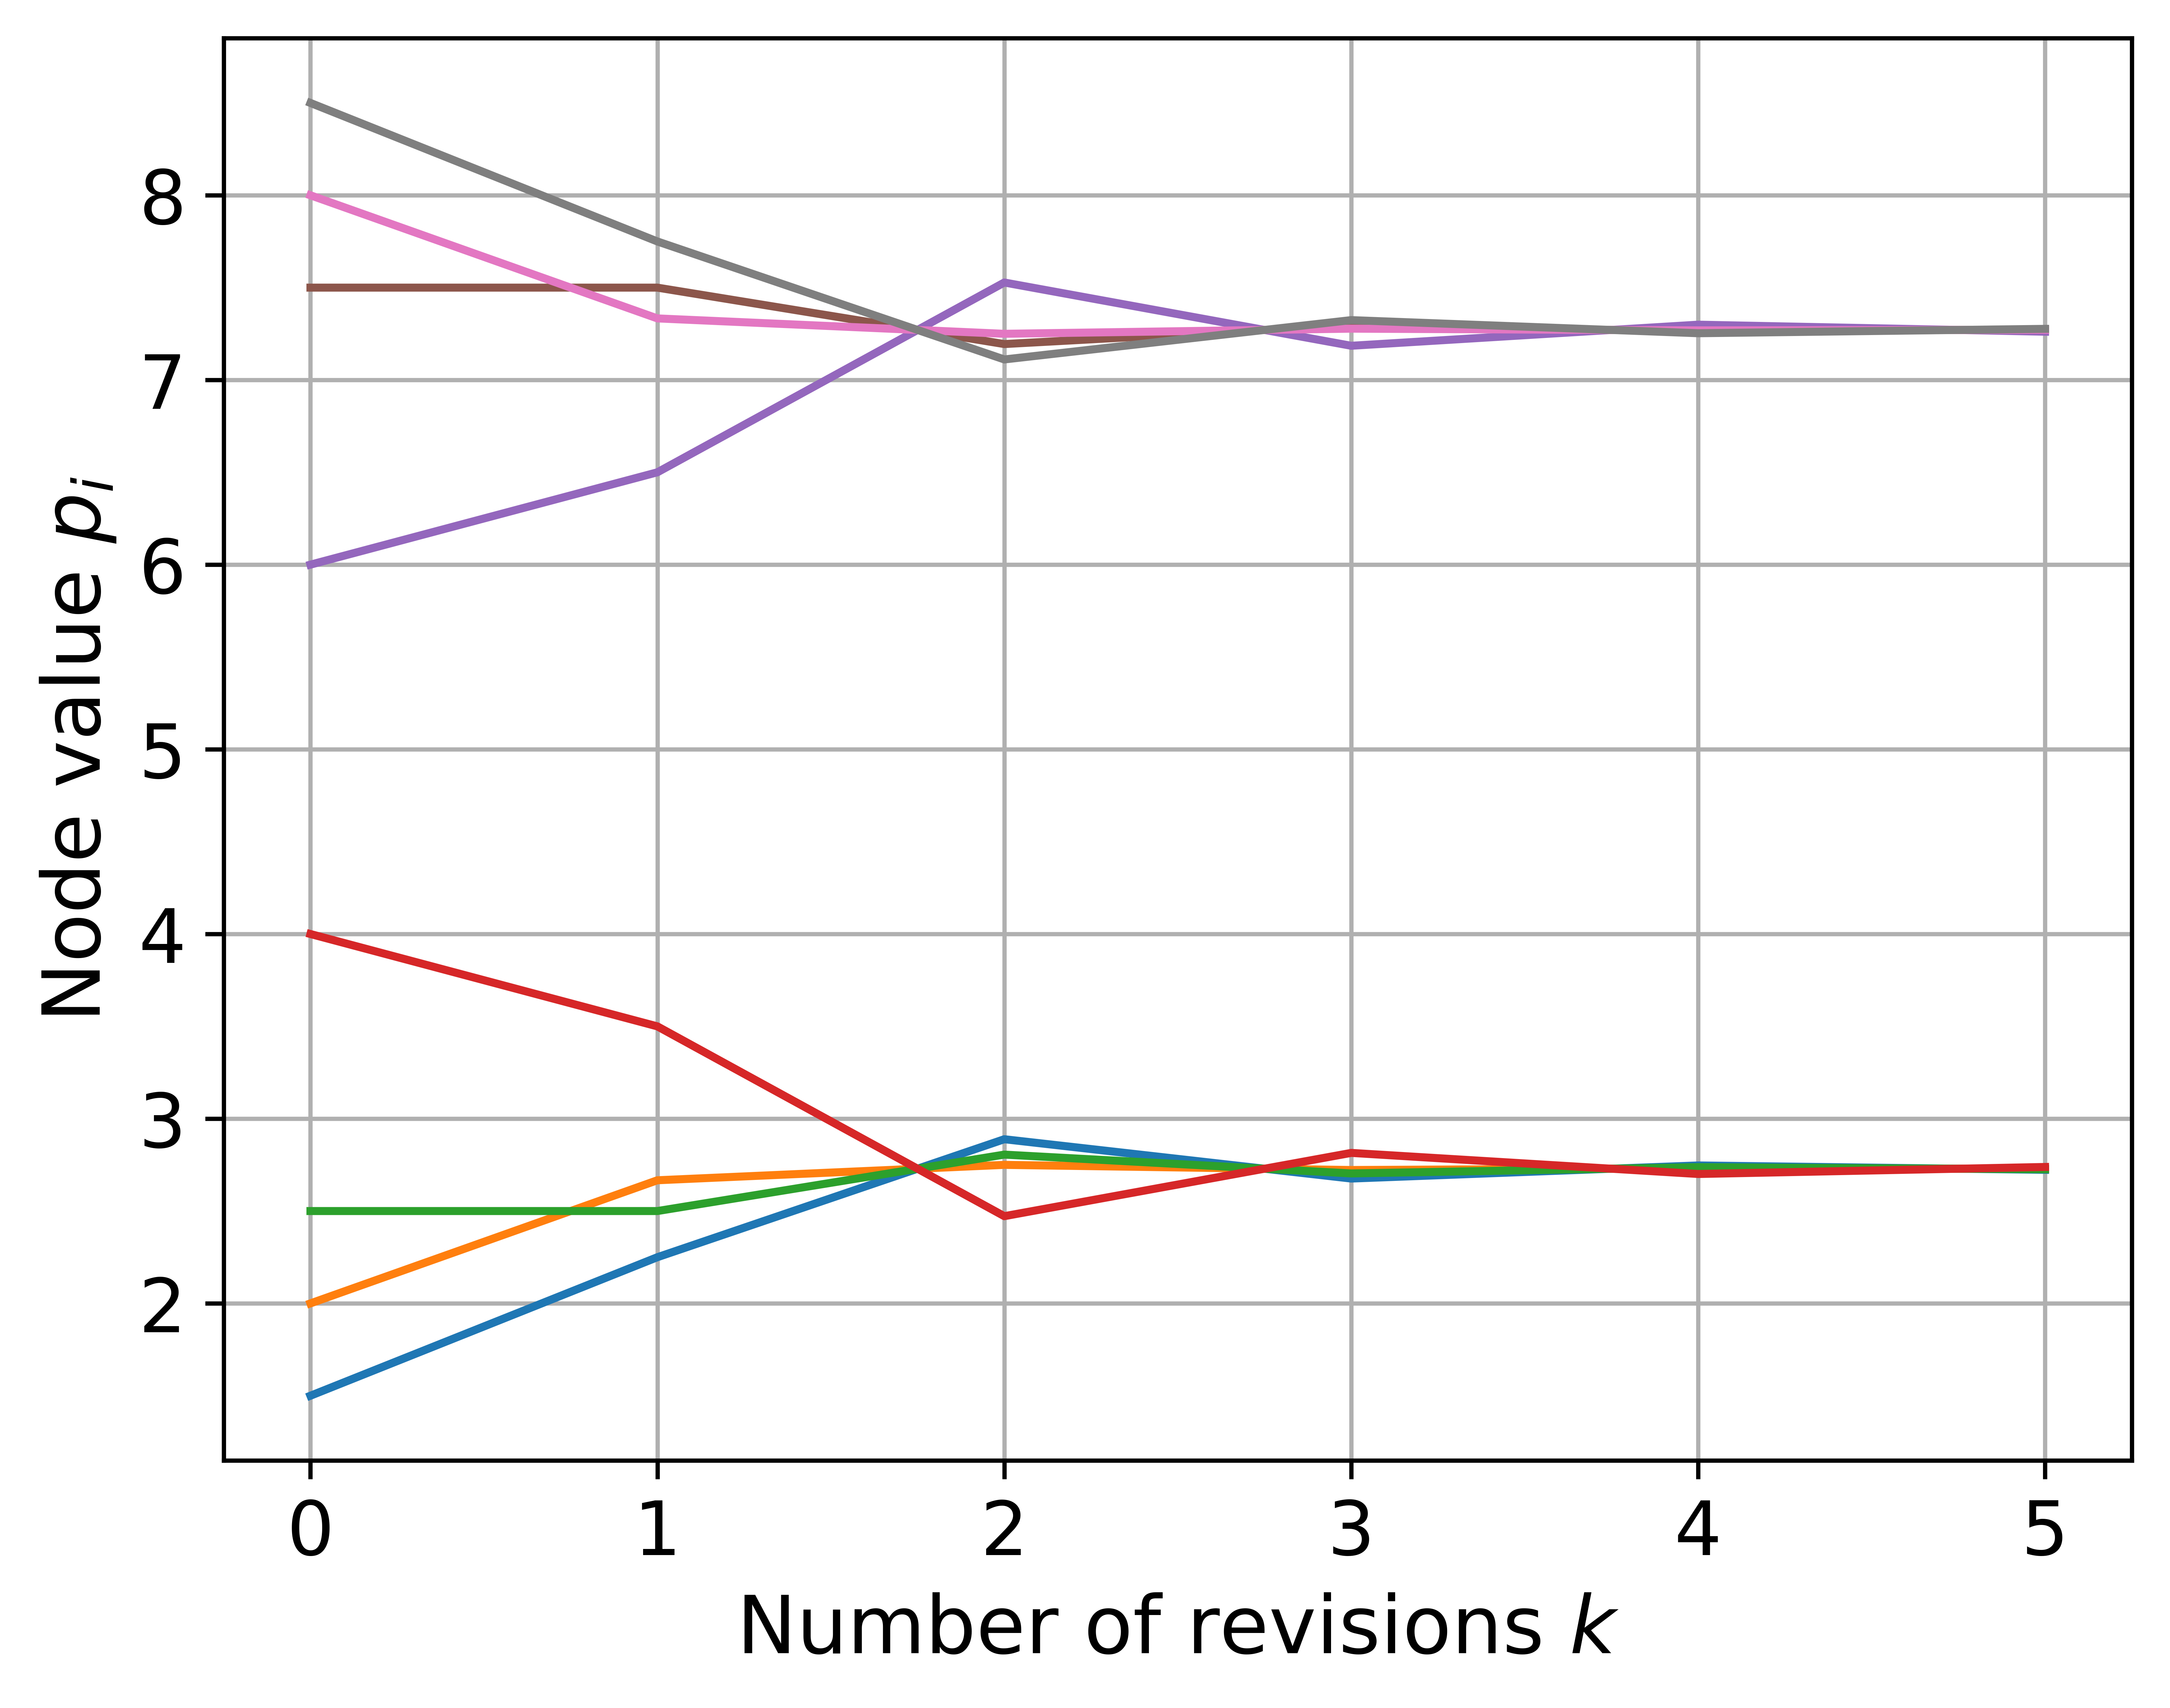
\includegraphics[scale= 0.4]{pictures/bounded_confs.png}
        \caption{The figure shows an instance of the Hegselmann-Krause model with the bounded confidence value $\epsilon = 2$.}
        \label{fig:bounded_conf}
\end{figure}




%Likelihood of breaking edge


% \subsection{Biased agents}
% To further simulate the phenomenon of favoring opinions that align closely with one's own, so-called biased agents could be introduced. In the DeGroot model this can implemented to a certain extent by setting the initial high weights in the matrix $\mat A$ for individuals who hold similar opinions. However, this does not guarantee, that this phenomenon is taken into consideration during the entire process. 

% Similarly to the approach presented in Subsection \ref{sec:bounded_conf}, this feature could be implemented by skewing the row vectors $a_i$ of the matrix $\mat A$ in every revision to favor individuals who hold opinions which align with $p_i$, i.e., assign higher values to individuals that have a low distance $|p_i-p_j|$.

\section{Conclusion and Outlook}
In this paper, we examined the DeGroot model to analyze the formation of opinions in groups. 
We then reproduced in \cref{th:semi_conv} under which conditions the model converges, as well as a sufficient condition (primitive matrices) and a necessary condition (existence of a globally reachable node) for a convergence towards a consensus. The paper also shows that only the left eigenvector $\vec{r^\T}$ and the vector of initial opinion values $\vec{p_0}$ are necessary to compute the consensus value. Moreover, we showed that the second largest eigenvector in magnitude $\lambda_{max}$ is a good measure for the convergence rate of the model. Furthermore, we looked at how the disagreement of graphs with multiple strongly connected subgraphs can be calculated and how the connectedness of a graph can be used as a further measure for the convergence rate. Lastly, we expanded on the DeGroot model by examining the additional features: \textit{susceptibility} and \textit{confidence bounds}.

In the future, further extensions that simulate other phenomena could be taken into account. For example, repulsive behavior ("negative weights") that allows for a change in the opposite direction of the other individuals opinion values \cite{chen2019opiniondynamicsbackfireeffect}, interrelated topics, as a subject rarely exists in isolation \cite{Parsegov_2017}, or a distinction between publicly versus privately expressed opinions (especially opinions on highly stigmatized topics, are often expressed only to certain individuals) \cite{Ye_2019}.


% The list of references is provided as `references.bib`
\bibliographystyle{unsrt}
\bibliography{IEEEabrv,references}

\end{document}